% Sample paper for the compile corpus: the bibliography is written by filecontents (so the
% compile writes a file in /work), cited through BibTeX, with a TikZ figure, maths, a table and
% cross-references. All names and references are made up.
\begin{filecontents}[overwrite]{refs.bib}
@article{example2024graphs,
  author  = {Example, Alex and Sample, Robin},
  title   = {Learning on Example Graphs},
  journal = {Journal of Made-Up Results},
  year    = {2024},
  volume  = {12},
  pages   = {1--20}
}
@inproceedings{sample2023trees,
  author    = {Sample, Robin},
  title     = {Trees That Do Not Exist},
  booktitle = {Proceedings of the Imaginary Conference},
  year      = {2023},
  pages     = {33--41}
}
\end{filecontents}
\documentclass[11pt]{article}
\usepackage[T1]{fontenc}
\usepackage{lmodern}
\usepackage{amsmath,amssymb}
\usepackage{graphicx}
\usepackage{booktabs}
\usepackage{tikz}
\usetikzlibrary{arrows.meta,positioning}
\usepackage[colorlinks=true]{hyperref}

\title{A Sample Paper on Example Graphs}
\author{Alex Example \and Robin Sample}
\date{January 2026}

\begin{document}
\maketitle

\begin{abstract}
We show that example graphs are useful for testing a compile service. Prior work on example
graphs~\cite{example2024graphs} and on trees~\cite{sample2023trees} motivates the study.
\end{abstract}

\section{Introduction}\label{sec:intro}
Let $G = (V, E)$ be a graph with $|V| = n$. The degree sum satisfies
\begin{equation}\label{eq:degree}
  \sum_{v \in V} \deg(v) = 2|E|.
\end{equation}
Equation~\eqref{eq:degree} and Figure~\ref{fig:pipeline} are referred to in Section~\ref{sec:results}.

\begin{figure}[ht]
  \centering
  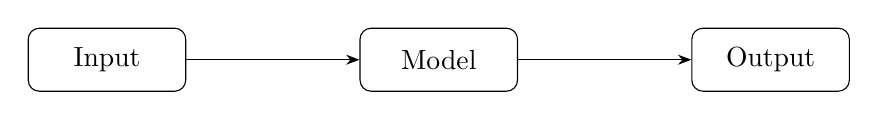
\begin{tikzpicture}[node distance=2.2cm, box/.style={draw, rounded corners, minimum width=2cm, minimum height=0.8cm}]
    \node[box] (in) {Input};
    \node[box, right=of in] (model) {Model};
    \node[box, right=of model] (out) {Output};
    \draw[-{Stealth}] (in) -- (model);
    \draw[-{Stealth}] (model) -- (out);
  \end{tikzpicture}
  \caption{The pipeline.}\label{fig:pipeline}
\end{figure}

\section{Results}\label{sec:results}
\begin{table}[ht]
  \centering
  \begin{tabular}{lrr}
    \toprule
    Method & Accuracy & Time (s) \\
    \midrule
    Baseline & 0.71 & 1.2 \\
    Ours     & 0.84 & 1.5 \\
    \bottomrule
  \end{tabular}
  \caption{Made-up results.}\label{tab:results}
\end{table}
Table~\ref{tab:results} lists the results.

\bibliographystyle{plain}
\bibliography{refs}
\end{document}
